%%% Local Variables:
%%% TeX-command-extra-options: "-shell-escape"
%%% mode: latex
%%% TeX-master: t
%%% End:
\documentclass{beamer}
\usepackage{caption}
\usepackage{minted}
\usepackage{tikz}
\usepackage{xcolor}
\usepackage{hyperref}
\usetikzlibrary{shapes.geometric, arrows}
\tikzstyle{startstop} = [rectangle, rounded corners, minimum width=3cm, minimum height=1cm,text centered, draw=black, fill=red!30]
\tikzstyle{io} = [trapezium, trapezium left angle=70, trapezium right angle=110, minimum width=1.5cm, minimum height=0.6cm, text centered, draw=black, fill=blue!30]
\tikzstyle{process} = [rectangle, minimum width=1.5cm, minimum height=0.5cm, text centered, draw=black, fill=orange!30]
\tikzstyle{decision} = [circle, radius=2.5cm, text centered, draw=black, fill=green!30]
\tikzstyle{arrow} = [thick,->,>=stealth]
\usepackage[labelformat=simple]{subcaption}

\usetheme{Singapore}
\title{Getting Started in Racket}
%\subtitle{in Racket}
%\author{Peter Campora}
%\institute{ULL}
%\date{\today}

%This lectures introduces Racket basics at a slow pace
\begin{document}
\begin{frame}
\titlepage
\end{frame}

\begin{frame}
  \frametitle{Your Lecturer's Apology}
  Before we start, a brief digression again. If something seems
  strange I want to you to \emph{think} about why it is strange
  or \emph{ask} about why it is strange. Same for if something is difficult.
  If something is difficult and it seems like it shouldn't be, congratulations!
  \textbf{You've found a research problem.}
  \begin{center}
    \includegraphics[width=0.35\textwidth]{images/GHH.jpg}
  \end{center}
  Also, I want you to think about whether aspects of programming are
  aesthetic, as the late G. H. Hardy claimed mathematics was.  
\end{frame}

\section{Arithmetic in Racket}
\begin{frame}
  \frametitle{Starting Dr. Racket}
  To start writing a Racket Program, we first open Dr. Racket and save a file.
  A fresh instance of Dr. Racket should look like:\\
  \pause
  \begin{center}
    \includegraphics[width=0.8\textwidth]{images/Dr-Racket-Empty.png}
  \end{center}

\end{frame}

\begin{frame}
  \frametitle{Handy Libraries to Include}
  We will frequently be using packages that were designed for the book that this course is based on: How to Design Programs (2e). Some
  handy packages include 2hdtp/image and 2htdp/universe.
  \begin{itemize}
  \item<2-> To include these, we use the \mintinline{racket}{require} expression as follows:
  \item<3-> \mintinline{racket}{(require 2htdp/image 2htdp/universe)}
  \item<4-> To load these packages so that we can play around in the interactions window, we hit the green run button at the top right.
  \item<5-> \includegraphics[width=0.9\textwidth]{images/run-button.png}
  \end{itemize}
\end{frame}

\begin{frame}
  \frametitle{Nifty Features}
  Last time I mentioned that Dr. Racket has some nifty features like the fact that it can render images and you can copy and paste images
  into it.
  \begin{itemize}
  \item<2-> Placing the cursor over an included function indicates what package it was included from.
  \item<3-> \includegraphics[width=0.7\textwidth]{images/function-arrow.png}
  \end{itemize}
\end{frame}

\begin{frame}
  \frametitle{Nifty Features (cont.)}
  Highlighting a package shows all of the functions from this package that are used in the program.
  \begin{itemize}
  \item<2-> \includegraphics[width=0.7\textwidth]{images/package-arrows.png}    
  \end{itemize}
\end{frame}

\defverbatim[colored]\script{
\begin{minted}{racket}
    #lang racket
    (require 2htdp/image 2htdp/universe)
    (circle 10 "solid" "blue")
    (rectangle 40 60 "solid" "green")
\end{minted}
}

\begin{frame}
  \frametitle{Dr. Racket for Scripting}
  Consider the following program:
  \begin{itemize}
  \item<1->  \script
  \item<2-> Hitting the run button gives us the following result in the interactions window
  \item<3-> \includegraphics[width=0.5\textwidth]{images/script-output.png}
  \item<4-> But enough about Dr. Racket, let's start talking about the Racket language!
  \end{itemize}
\end{frame}

\begin{frame}
  \frametitle{Relearning Arithmetic}
  \begin{center}
    \includegraphics[width=0.7\textwidth]{images/arithmetic.jpg}
  \end{center}
\end{frame}

\begin{frame}
  \frametitle{Arithmetic Revisited}
  Warning! The start of this lecture will be a bit boring since it introduces
  the basic elements of Racket--starting with how to do arithmetic.
  \begin{itemize}
  \item<2-> \mintinline{racket}{(+ 1 1)}
  \item<3-> Just imagine for each new pair of parentheses that you put the operator
    between each spaced element.
  \item<4-> Evaluate left to right, and then inner parentheses naturally evaluate first: \mintinline{racket}{(+ 1 (+ 1 (+ 1 1) 2) 3 4 5)}
  \item<5-> == \mintinline{racket}{(+ 1 (+ 1 2 2) 3 4 5)}
  \item<6-> == \mintinline{racket}{(+ 1 5 3 4 5)}
  \item<7-> == \mintinline{racket}{18}
  \end{itemize}
\end{frame}

\begin{frame}
  \frametitle{Arithmetic Revisited (cont)}
  \begin{itemize}
  \item<1-> Primitive form is \mintinline{racket}{(operator number+)}
  \item<2-> A list of useful operators:  +, -, *, /, abs, add1, ceiling, denominator, expt, floor, gcd, log, max, numerator, quotient, random, remainder, sqr, and tan
  \item<3-> Racket has an extensive \emph{numeric tower}.
  \item<4-> What would \mintinline{racket}{(/ 4 3)} produce in Java?
  \item<5-> 1.33... as a floating point value.
  \item<6-> Instead of producing a float, Racket produces $\frac{4}{3}$.
  \item<7-> To get a float, you need to use \mintinline{racket}{(exact->inexact (/ 4 3))}
  \item<8-> Other operations like \mintinline{racket}{(sqrt 2)} immediately produce floats.
  \item<9-> Let's play around with this a bit!
  \end{itemize}
\end{frame}

\begin{frame}
  \frametitle{Defining Constants}
  Defining constants is an important part of many programs. Let's take
  a look at how to define global constants.
  \begin{itemize}
  \item<2-> To define a constant, we simply write expressions of the form:
    \mintinline{racket}{(define my-variable expression)} 
  \item<3-> To define my age we would write:
    \mintinline{racket}{(define object-mass 20)}
  \item<4-> But of course we can write more complicated expressions
    to define constants: \mintinline{racket}{(define c (* 3 (expt 10 8)))}
  \item<5-> The order of defining constants matters. To define the energy of
    our object we put this constant definition last:
    \mintinline{racket}{(define object-energy (* object-mass (sqr c))}
  \item<6-> Let me demonstrate the error that arises otherwise.
  \end{itemize}
\end{frame}

\begin{frame}
  \frametitle{Arithmetic of Strings}
  You may think of arithmetic involving integers or real numbers, but
  we can also have arithmetic on strings!
  \begin{itemize}
  \item<2-> String concatenation is one fundamental operation: \mintinline{racket}{(string-append "Hello " "World")} $\hookrightarrow$
    \mintinline{racket}{"Hello World"}
  \item<3-> We can give it multiple arguments: \mintinline[fontsize=\footnotesize]{racket}{(string-append "What a " "lovely " "day" " for Racket!")} $\hookrightarrow$ \mintinline{racket}{"What a lovely day for Racket!"}
  \item<4-> The identity element for string-append is "":
    \mintinline{racket}{(string-append "foo" "")} $\hookrightarrow$
    \mintinline{racket}{"foo"}
  \item<5-> We can get the length of strings: \mintinline{racket}{(string-length "abc")} $\hookrightarrow$ \mintinline{racket}{3}
  \item<6-> We can extract a specific character: \mintinline{racket}{(string-ref "abc" 0)} $\hookrightarrow$ \mintinline{racket}{"a"}
  \item<7-> We can take a substring of a string: \mintinline{racket}{(substring "foobar" 0 3)} $\hookrightarrow$ \mintinline{racket}{"foo"}
  \item<8-> Can convert numbers to strings: \mintinline{racket}{(number->string 42)} $\hookrightarrow$ \mintinline{racket}{"42"}
  \end{itemize}
\end{frame}

\begin{frame}
  \frametitle{Arithmetic of Images}
  A lot of functions are available for manipulating images:
  \begin{itemize}
  \item<2-> Circles: \mintinline{racket}{(define my-circle (circle 10 "outline" "green"))}
  \item<3-> Rectangles: \mintinline{racket}{(define my-rectangle (rectangle 10 20 "solid" "red"))}
  \item<4-> Get the height of an image: \mintinline{racket}{(image-height my-rectangle)}
  \item<5-> Or the width: \mintinline{racket}{(image-width my-rectangle)}
  \item<6-> You can layer images with overlay: \mintinline{racket}{(overlay my-circle my-rectangle)}
  \item<7-> See also \mintinline{racket}{overlay/xy} and \mintinline{racket}{overlay/align}
  \item<8-> And you can put images over each other (see \mintinline{racket}{above})
    or next to each other (see \mintinline{racket}{beside})
  \end{itemize}
\end{frame}

\begin{frame}
  \frametitle{Arithmetic of Images (cont.)}
  The starting points for drawing images typically involves the functions below:
  \begin{itemize}
  \item<2-> \mintinline{racket}{empty-scene}, \mintinline{racket}{place-image},
    and \mintinline{racket}{scene+line}
  \item<3-> To create an empty-scene:
    \mintinline{racket}{(define canvas (empty-scene 100 100 "white"))}
  \item<4-> To place an image into the scene:
    \mintinline{racket}{(place-image my-rectangle 50 50 canvas)}  
  \item<5-> We can directly copy this image into Dr. Racket: 
\includegraphics[width=0.05\textwidth]{images/cat.png}    
  \end{itemize}
\end{frame}

\begin{frame}
  \frametitle{Arithmetic Laws}
  \begin{center}
    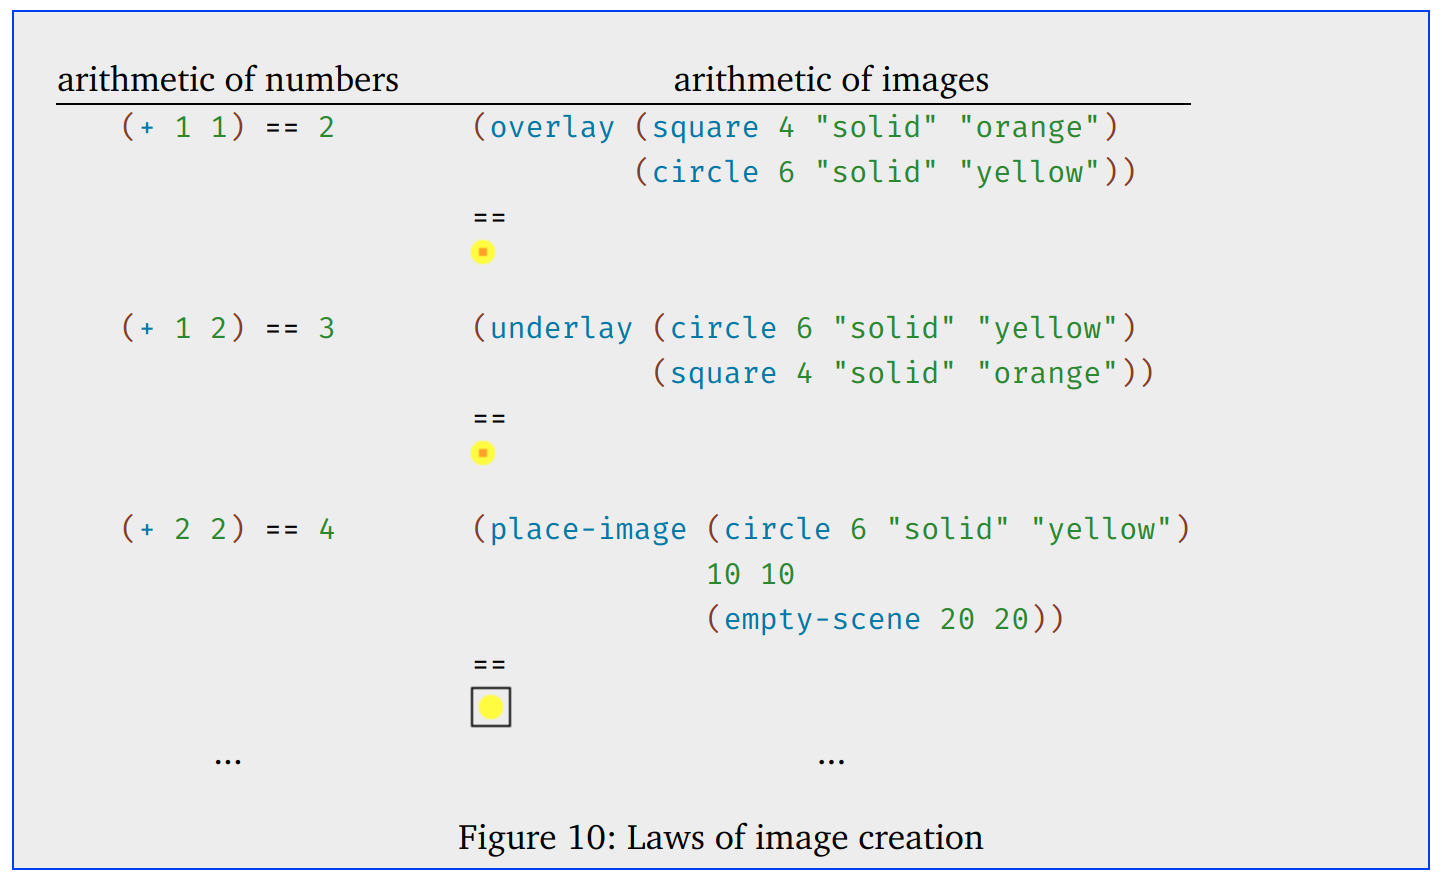
\includegraphics[width=0.7\textwidth]{images/Arithmetic-Images.png}
  \end{center}
\end{frame}

% \defverbatim[colored]\schemeTrue{
% \begin{minted}{racket}
%   #t
% \end{minted}
% }

\defverbatim[colored]\cond{
\begin{minted}{racket}
    (cond 
      [(> x 0) 1]
      [(= x 0) 0]
      [else -1])
\end{minted}
}

\begin{frame}
  \frametitle{Arithmetic of Booleans}
  Boolean Arithmetic should look familiar to all of you.
  \begin{itemize}
  \item<2-> The primitive boolean values are: 
    \text{\#t} and \text{\#f}
  \item<3-> The functions \mintinline{racket}{and}, \mintinline{racket}{or}, and
    \mintinline{racket}{not} do exactly what you expect
  \item<4-> We can write conditional expressions with the form:
    \mintinline{racket}{(if test-exp true-branch else-branch)}
  \item<5-> \item<5-> Here's an example:
    \mintinline{racket}{(if (< 0 1) 1 2)} $\hookrightarrow$ \mintinline{racket}{2}
  \item<5-> What does the following expression evaluate to?
    \mintinline{racket}{(+ 1 (if (< 0 1) 1 2))}
  \item<6-> When we have more conditions we use \mintinline{racket}{cond}:
    \cond
  \end{itemize}  
\end{frame}

\defverbatim[colored]\catProgram{
\begin{minted}{racket}
    (define cat-height (image-height cat))
    (define cat-width (image-width cat))
    
    (if (>= cat-height cat-width) 
        "long cat!" 
        "heckin chonker!")
\end{minted}
}

\begin{frame}
  \frametitle{Our First Program}
  Let's write a program to classify whether this cat is a long cat or a heckin
  chonker!
  \begin{center}
    
\includegraphics[width=0.1\textwidth]{images/cat.png}    
  \end{center}
  \begin{itemize}
  \item<2-> It should be a long cat if its height (tail height counts) is higher
    than its width.
  \item<3-> Help me write it! We're going to need
    \mintinline{racket}{image-height} and \mintinline{racket}{image-width}.
  \item<4-> Here it is: \catProgram
  \end{itemize}
\end{frame}

\begin{frame}
  \frametitle{Predicates}
  Predicates are a short way of saying boolean valued function. Let's take
  a look at some important predicates in Racket.
  \begin{itemize}
  \item<2-> We can check if something is a number with \mintinline{racket}{number?}
  \item<3-> \mintinline{racket}{(number? 2)}, \mintinline{racket}{(number? 2.3)}, and \mintinline{racket}{(number? 2/3)} all return true
  \item<4-> Surprisingly \mintinline{racket}{(rational? 2)}, \mintinline{racket}{(rational? (sqrt 2))}, and \mintinline{racket}{(rational? 2/3)} all return true too.
  \item<5-> \includegraphics[width=0.3\textwidth]{images/science-liar.jpg}
  \item<6-> Use \mintinline{racket}{(exact? (sqrt 2))} or \mintinline{racket}{(inexact? (sqrt 2))}
  %\item<7-> There are many other predicates: \mintinline{racket}{real?},
  %  \mintinline{racket}{boolean?}, \mintinline{racket}{image?},
  %  \mintinline{racket}{string?}, \mintinline{racket}{complex?}, ...
  \end{itemize}
\end{frame}

\defverbatim[colored]\predicateSkeleton{
\begin{minted}{racket}
    (cond
      [(... in) ...]
      ...)
\end{minted}
}

\defverbatim[colored]\predicatePartial{
\begin{minted}{racket}
    (cond
      [(string? in) ...]
      ...)
\end{minted}
}
\defverbatim[colored]\predicateFinal{
\begin{minted}[fontsize=\footnotesize]{racket}
    (cond 
        [(string? in) (string-length in)]
    	[(and (number? in) (> in 0)) (sub1 in)]
    	[(image? in) (* (image-height in) (image-width in))]
    	[else in])
\end{minted}
}
\begin{frame}
  \frametitle{Programming With Predicates}
  Create an expression that converts the value of \mintinline{racket}{in} to a positive number. For a String, it determines how long the String is; for an Image, it uses the area; for a Number, it decrements the number by 1, unless it is already 0 or negative; for true it uses 10 and for false 20.
\begin{itemize}
\item<2-> Let's diagram this out.
\item<3-> Here is our skeleton: \predicateSkeleton
%\item<4-> \predicatePartial
\item<4-> Here is our final version: \predicateFinal
\end{itemize}

\end{frame}

% \begin{frame}
%   \frametitle{Booleans and Conditionals}
%   \begin{itemize}
%   \item<2-> The structure of basic conditional statements:
%     \mintinline{racket}{(if test-exp true-branch else-branch)}
%   \item<3-> \mintinline{racket}{(if #t 1 2) ;;produces 1}
%   \item<4-> Can use it as an argument to other operations:
%     \mintinline{racket}{(+ 1 (if #t 1 2))}
%   \item<5-> This means that conditionals in Racket are expressions.
%   \item<6-> If we don't want to nest if-expressions, we use \mintinline{racket}{cond}
%   \item<7-> \mintinline{racket}{(cond [test-1 result-1] ...[test-n result-n])}
%   \item<8-> Let's record the sign of some integer x: \cond
%   \end{itemize}
% \end{frame}


\section{From Arithmetic to Functions}
\begin{frame}
  \frametitle{Our Bread and Butter}
  \begin{center}
    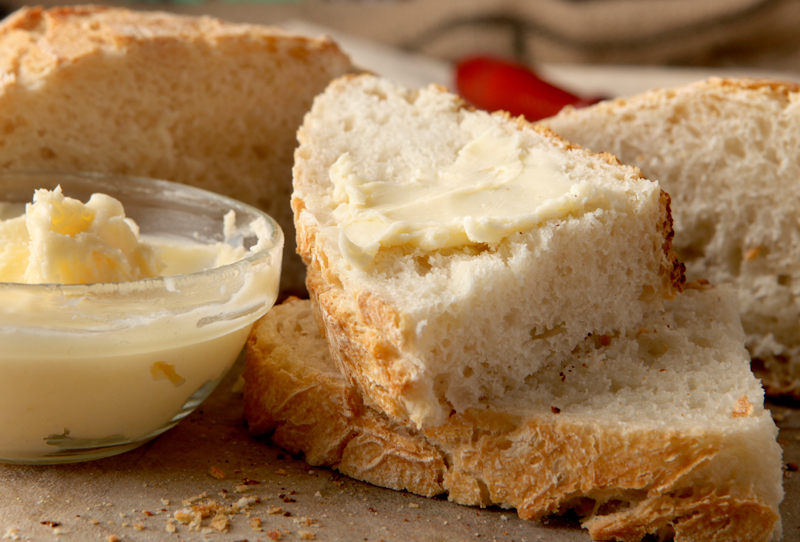
\includegraphics[width=0.4\textwidth]{images/bread-butter.jpg}
  \end{center}
  \begin{itemize}
  \item<2-> Yum!
  \item<3-> Functions are the bread and butter of functional programming, so let's get that bread!
  \item<4-> \huge But first, what is a function?
  \end{itemize}
\end{frame}



\begin{frame}
  \frametitle{The Algebra of Programming}
  \begin{figure}
    \begin{subfigure}{0.45\textwidth}
      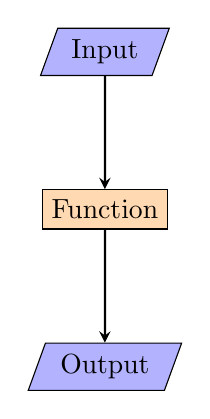
\begin{tikzpicture}[node distance=2cm]
        % \node (start) [startstop] {Start};
        \node (in1) [io] {Input};
        \node (pro1) [process, below of=in1] {Function};
        \node (out1) [io, below of=pro1] {Output};
        \draw [arrow] (in1) -- (pro1);
        \draw [arrow] (pro1) -- (out1);
      \end{tikzpicture}
    \end{subfigure}
    \pause
    \begin{subfigure}{0.45\textwidth}
      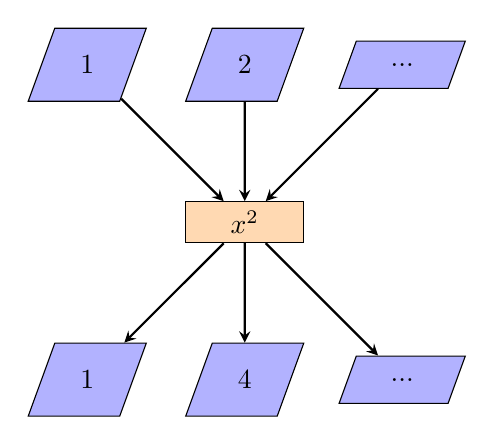
\begin{tikzpicture}[node distance=2cm]
        % \node (start) [startstop] {Start};
        \node (in1) [io] {2};        
        \node (in2) [io, right of=in1] {...};
        \node (in3) [io, left of=in1] {1};
        \node (pro1) [process, below of=in1] {$x^2$};

        \node (out1) [io, below of=pro1] {4};
        \node (out2) [io, right of=out1] {...};
        \node (out3) [io, left of=out1] {1};
        
        \draw [arrow] (in1) -- (pro1);
        \draw [arrow] (in2) -- (pro1);
        \draw [arrow] (in3) -- (pro1);
        
        \draw [arrow] (pro1) -- (out1);
        \draw [arrow] (pro1) -- (out2);
        \draw [arrow] (pro1) -- (out3);
      \end{tikzpicture}
    \end{subfigure}
  \end{figure}
\end{frame}

\defverbatim[colored]\arrayList{
\begin{minted}{Java}
import java.util.ArrayList;
class Main {
  public static void main(String[] args) {
    System.out.println("Hello world!");
    ArrayList<Integer> alist = new ArrayList<Integer>();
    alist.add(1);
    alist.add(2);
    System.out.println(alist.remove((Object)1));
    System.out.println(alist.remove((Object)1));
  }
}
\end{minted}
}

\begin{frame}
  \frametitle{Definitions and Misconceptions}
  Mathematicians and Computer Scientists \emph{love} definitions.
  \begin{itemize}
    \item<2-> A \textbf{relation} is a set of ordered pairs.
    \item<3-> A \textbf{function} is a relation for which each value from the set the first components of the ordered pairs is associated with exactly one value from the set of second components of the ordered pair.
    \item<4-> Let's consider what isn't a function.
    \item<5-> \mintinline{Java}{aList.remove((Object)1);//assume ArrayList<Integer>}
    \item<6-> Repeatedly calling this method with the input produces
      different results.
    \item<7-> So this is a relation and not a function!
  \end{itemize}
\end{frame}

\begin{frame}
  \frametitle{A Difference in Design 1}
  Let's take a look at an idealized model of object oriented design:
  \pause
  \begin{center}
    \includegraphics[width=0.65\textwidth]{images/oo-design.png}
  \end{center}
\end{frame}

\begin{frame}
  \frametitle{A Difference in Design 2}
  Functional design is just about composing a series of functions:
  \pause
  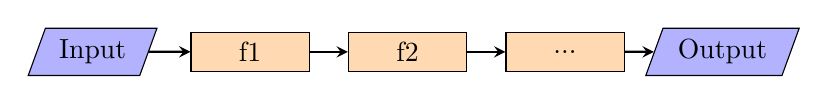
\begin{tikzpicture}[node distance=2cm]
    % \node (start) [startstop] {Start};
    \node (in1) [io] {Input};
    \node (pro1) [process, right of=in1] {f1};
    \node (pro2) [process, right of=pro1] {f2};
    
    \node (pro3) [process, right of=pro2] {...};
    \node (out1) [io, right of=pro3] {Output};
    \draw [arrow] (in1) -- (pro1);
    \draw [arrow] (pro1) -- (pro2);
    \draw [arrow] (pro2) -- (pro3);
    \draw [arrow] (pro3) -- (out1);
  \end{tikzpicture}
  \begin{itemize}
  \item<2-> Our focus is on how to model the input and output data.
  \item<3-> From there, our program is a series of functions that transform
    the input data into the output data.
  \item<4-> We carefully segregate \emph{effectful} code from our pure functions.
  \item<5-> \includegraphics[width=0.2\textwidth]{images/haskell.png}
  \end{itemize}
      
\end{frame}

\begin{frame}
  \frametitle{Getting Our Hands Dirty}
  When we defined constants in Racket, we used the form:
  \mintinline{racket}{(define constant exp)}
  \begin{itemize}
  \item<2-> To define functions: \mintinline{racket}{(define (fun-name params...) fun-body)}
  \item<3-> To define $square(x) = x^2$:
    \mintinline{racket}{(define (square x) (* x x))}
  \item<4-> For a function of two parameters:
    \mintinline{racket}{(define (add x y) (+ x y))}
  \end{itemize}
\end{frame}

\begin{frame}
  \frametitle{Debugging Incorrect Code}
  Consider the following function:
  \mintinline{racket}{(define (my-not b) (not b 1))}
  \begin{itemize}
  \item<2-> What happens when we make the following call? \mintinline{racket}{(my-not t)}
  \item<3-> \includegraphics[width=0.4\textwidth]{images/debugger.png}
  \item<4-> Let's play around with the debugger.
  \end{itemize}
\end{frame}

\begin{frame}
  \frametitle{Defining Basic Functions}
  Defining the distance to the origin $f(x, y) = \sqrt{x^2 + y^2}$ is simple:
  \begin{itemize}
  \item<2-> \mintinline{racket}{(define (distance x y) (sqrt (+ (sqr x) (sqr y))))}
  \item<3-> Defining implication $p \Rightarrow q$ as a function is straightforward.
  \item<4-> Recall the truth table for implication:\\
      \begin{tabular}{ l | l | l }
      $p$ & $q$ & $p \Rightarrow q$ \\ \hline
      f & f & t\\
      t & f & f\\
      f & t & t\\
      t & t & t\\
    \end{tabular}
  \item<5-> \mintinline{racket}{(define (==> p q) (or (not p) q))}
  \item<6-> Here is a secret: \mintinline{racket}{(p . ==> . q)}
  \item<7-> Place dots around a function to use it infix.    
  \end{itemize}
\end{frame}


\begin{frame}
  \frametitle{Baby's First Homework}
  Homework 1. Several programs involve string functions, so see the: \href{https://docs.racket-lang.org/reference/strings.html}{\textcolor{blue}{string documentation}}.
  \begin{enumerate}
  \item Define the function cvolume, which accepts the length of a side of an equilateral cube and computes its volume. If you have time, consider defining csurface, too.
  \item Define the function string-first, which extracts the first character from a non-empty string. (see \mintinline{racket}{string-ref})
  \item Define the function string-last, which extracts the last character from a non-empty string. 
  \item Define the function image-area, which counts the number of pixels in a given image. (see \mintinline{racket}{image-height} and \mintinline{racket}{image-width})
  \item Define the function image-classify, which consumes an image and conditionally produces "tall" if the image is taller than wide, "wide" if it is wider than tall, or "square" if its width and height are the same. (hint see cat chonker program)  
  \end{enumerate}
\end{frame}

\begin{frame}
  \frametitle{Baby's First Homework (cont.)}
  \begin{enumerate}
    \setcounter{enumi}{5}
 \item Define the function string-join, which consumes two strings and appends them with "\_" in between. (see \mintinline{racket}{substring})
  \item Define the function string-insert, which consumes a string str plus a number i and inserts "\_" at the ith position of str. Assume i is a number between 0 and the length of the given string (inclusive). Ponder how string-insert copes with "".
  \item  Define the function string-delete, which consumes a string plus a number i and deletes the ith position from str. Assume i is a number between 0 (inclusive) and the length of the given string (exclusive). Can string-delete deal with empty strings? 
  \end{enumerate}
\end{frame}

\begin{frame}
  \frametitle{So, What About \emph{Real} Programs?}
  By now, you guys are probably wanting to write more than just single
  function definitions. So let's talk about writing \emph{scripts}, which
  we'll refer to as batch programs.
  \begin{itemize}
  \item<2-> We can design batch programs as a bunch of composed functions
    that are passed input data.
  \item<3-> Typically this input data will come from the outside world, or
    we will have certain functions interactions with the external world.
  \item<4-> A lot of the times batch programs interact with a user to get
    some basic input and read or write to files.
  \end{itemize}
\end{frame}

\begin{frame}
  \frametitle{Designing Batch Programs}
  So let's take a look at how we can write scripts.
  \begin{itemize}
  \item<2-> Let's consider writing a program that fills a letter template with different names. I want to fill in the name of the person that I request the letter
    from, and the name of the company to send it to. While we're at it, let's
    make it so I can sign the letter with different names.
  \item<3-> \includegraphics[width=0.4\textwidth]{images/letter.jpg}
  \item<4-> The anatomy of a letter consists of opening, body, and closing that
    need to be parameterized by names.  
  \end{itemize}
\end{frame}

\defverbatim[colored]\body{
\begin{minted}[fontsize=\footnotesize]{racket}
(define (body company)
  (string-append "I am applying for a job at " company "..."))
\end{minted}
}

\defverbatim[colored]\closing{
\begin{minted}[fontsize=\footnotesize]{racket}
(define (closing signature-name)
  (string-append "Sincerely," "\n\n" signature-name "\n"))
\end{minted}
}

\defverbatim[colored]\letter{
\begin{minted}[fontsize=\footnotesize]{racket}
(define (letter recipient company signature-name)
  (string-append
    (opening recipient)
    "\n\n"
    (body company)
    "\n\n"
    (closing signature-name)))
\end{minted}
}
\begin{frame}
  \frametitle{Our First Batch Program}
   Let's start with the opening:
   \mintinline{racket}{(define (opening fst) (string-append "Dear " fst ","))}
   \pause
  From here, let's move onto making a function to insert a company in the body:
  \body
  \pause
  Here's the closing:
  \closing
  \pause
  Finally, the main ``script'' part of our program is:
  \letter
\end{frame}

\begin{frame}
  \frametitle{What about IO?}
  Our program was a pure function since it always produces the same letter
  when called with the same input. But in reality, we might want to prompt
  the user for input and display the letter as output. For now, we will just show
  how to print the letter.
  \begin{itemize}
  \item<2-> To use IO we must first add this to our program:
    \mintinline{racket}{(require 2htdp/batch-io)}
  \item<3-> \mintinline[fontsize=\footnotesize]{racket}{(write-file 'stdout (letter "Mr. Campora" "WPI" "Bob Trufant"))}
  \item<4-> So, our program is structured as a call to one impure procedure after
    the composition of multiple pure functions did all of the work.
  \item<5-> One of the main goals of functional programming is to separate the
    pure core logic of the program from the effectful parts.    
  \end{itemize}
\end{frame}

\begin{frame}
  \frametitle{More About Structure}
  \begin{center}
    \includegraphics[width=0.4\textwidth]{images/FunctionalStructure.pdf}
  \end{center}
  \begin{itemize}
  \item<2-> Functional programming is about embedding a referentially transparent
    core into a layer that feeds data in and out of the stateful world.
  \item<3-> This really aids testing, as you should be able to write tests for
    the majority of the functions in the pure core. We'll discuss testing later.
  \item<4-> You should design your programs so that each piece of
    (repeatable) functionality is separated into its own function.
  \end{itemize}
\end{frame}

\begin{frame}
  \frametitle{Why Many Functions?}
  To illustrate the importance of writing many functions, let's consider
  writing a program to calculate the profit of a theater with respect to
  ticket cost and attendance.
  \pause
  \\ \\
  \textbf{Sample Problem} The owner of a monopolistic movie theater in a small town has complete freedom in setting ticket prices. The more he charges, the fewer people can afford tickets. The less he charges, the more it costs to run a show because attendance goes up. In a recent experiment the owner determined a relationship between the price of a ticket and average attendance.
  \pause
  \begin{center}
    \includegraphics[width=0.4\textwidth]{images/Monopoly.jpg}
  \end{center}
\end{frame}

\begin{frame}
  \frametitle{Making Other People Money}
  At a price of \$5.00 per ticket, 120 people attend a performance. For each 10-cent change in the ticket price, the average attendance changes by 15 people. That is, if the owner charges \$5.10, some 105 people attend on the average; if the price goes down to \$4.90, average attendance increases to 135. Let’s translate this idea into a mathematical formula:
  \pause
  Let's not worry about mathematical modeling too much, though  it's an important
  part of programming.
  \\ \\
  \pause
  $\text{avg attendance}=120\text{people}-\frac{\text{\$new-price}-\$5}{\$0.1} \cdot 15 \text{people}$
  \\ \\
  \pause
  We also need to consider the cost of putting on the show. There is a flat \$180
  cost to put on the show and also a \$0.04 cost per attendee.
\end{frame}

\defverbatim[colored]\cost{
\begin{minted}[fontsize=\footnotesize]{racket}
     (define (cost ticket-price)
       (+ 180 (* 0.04 (attendees ticket-price))))
\end{minted}
}

\defverbatim[colored]\attendees{
\begin{minted}[fontsize=\footnotesize]{racket}
     (define (attendees ticket-price)
       (- 120 (* (- ticket-price 5.0) (/ 15 0.1))))
\end{minted}
}
\begin{frame}
  \frametitle{Calculating}
  Let's look back at the descriptions and see what functions naturally arise
  out of the definitions. Let's sketch this out on the board before we write code.
  \begin{itemize}
  \item<2-> The cost is a pretty easy function to define.
  \item<3-> Calculate the cost: \cost
  \item<4-> But notice that this depends on a function that computes the number
    of attendees for a given ticket price!
  \item<5-> Calculate the number of attendees: \attendees    
  \end{itemize}
\end{frame}

\defverbatim[colored]\revenue{
\begin{minted}{racket}
     (define (revenue ticket-price)
       (* ticket-price (attendees ticket-price)))
\end{minted}
}

\defverbatim[colored]\profit{
\begin{minted}{racket}
     (define (profit ticket-price)
       (- (revenue ticket-price)
          (cost ticket-price)))
\end{minted}
}

\begin{frame}
  \frametitle{Calculating (cont.)}
  Equipped with a function to calculate the number of attendees,
  we can calculate the revenue.
  \begin{itemize}
  \item<2-> Calculate revenue: \revenue
  \item<3-> And with revenue in hand, we can calculate profit.
  \item<4-> Profit: \profit    
  \end{itemize}
\end{frame}

\defverbatim[colored]\badProgram{
\begin{minted}{racket}
  (define (profit price)
   (- (* (+ 120
           (* (/ 15 0.1)
              (- 5.0 price)))
        price)
     (+ 180
        (* 0.04
           (+ 120
              (* (/ 15 0.1)
                 (- 5.0 price)))))))
\end{minted}
}

\begin{frame}
  \frametitle{Better Than The Alternative?}
  We can compare our series of functions to one function that directly computes
  the profit, and see the advantage in how we designed our program.
  \pause
  \badProgram
\end{frame}

\begin{frame}
  \frametitle{Phew!}
  \begin{center}
    \includegraphics[width=0.7\textwidth]{images/jordan.jpg}
  \end{center}
\end{frame}

\begin{frame}
  \frametitle{But Were There Still Problems?}
  The original version of the program was much better than the new version, but
  there are still some issues that need to be addressed.
  \begin{enumerate}
  \item<2-> There were still plenty of magic numbers that should be refactored into variables
  \item<3-> There was a lack of comments explaining how we got to the behavior of
    the functions and how they should be used.
  \item<4-> In general the code doesn't communicate how it was designed
  \end{enumerate}
\end{frame}

\begin{frame}
  \frametitle{Wishing For Metric Intuition}
  \begin{center}
    \includegraphics[width=0.55\textwidth]{images/metric-system.jpg}
  \end{center}
\end{frame}

\begin{frame}
  \frametitle{A Basic File IO Program}
  We will consider writing a simple program that converts Celsius temperatures to Fahrenheit, by reading from a file ``C.txt''
  and writing to a file ``F.txt''. Let's diagram out the structure of our application. What is the pure layer and what happens
  in the IO layer?
\end{frame}

\begin{frame}
  \frametitle{Back to Batch Programs}
  As defined earlier, batch programs are scripts that consume input from the
  user and then use a series of composed functions to accomplish some task.
  A common type involves File I/O, so I'll give a program that reads from and
  writes to a file.
  \begin{itemize}
  \item<2-> To read from ``foo.txt'' use: \mintinline{racket}{(read-file "foo.txt")}
  \item<3-> To write ``bar'' into ``foo.txt'' use: \mintinline{racket}{(write-file "foo.txt" "bar")}
  \item<4-> Let's write our temperature converting program now. Where should we start? 
  \end{itemize}  
\end{frame}

\defverbatim[colored]\convert{
\begin{minted}[fontsize=\footnotesize]{racket}
     (define (convert in out)
      (write-file out
        (string-append
          (number->string
            (C->F
              (string->number
                (read-file in))))
           "\n")))
\end{minted}
}

\begin{frame}
  \frametitle{A Quick Batch Program}
  First let's define the Celsius to Fahrenheit function:
  \begin{itemize}
  \item<2-> \mintinline{racket}{(define (C->F temp) (+ (* 9/5 temp) 32))}
  \item<3-> Unfortunately, with the current languages features we've introduced,
    the following definition isn't that elegant: \convert
  \item<4-> The most important things to note here are the converting between
    numbers and strings in the program.
  \item<5-> We will return to batch programs later, but for now we move to interactive programs.
  \end{itemize}
\end{frame}

\section{Interactive Programs}
\begin{frame}
  \frametitle{Let's Interact!}
  Circuits aren't so interesting (for Computer Scientists) in and of themselves.
  \\\\
  \pause
  They take in current (or lack thereof) as input and produce current (ditto) as output.
  \\\\
  \pause
  But CPUs allow for some more complicated behavior, and the first program  that is usually installed is the operating system (besides BIOS).
  \\\\
  \pause
  An operating system is essentially one big event driven program that is
  designed for continuous interaction.
  \\\\
  \pause
  Let's diagram this out and relate it to the type of programs we will soon
  be writing.
\end{frame}

\begin{frame}
  \frametitle{Event Structure In General}
  \begin{center}
    \includegraphics[width=0.75\textwidth]{images/Event_Driven.jpg}
  \end{center}
\end{frame}

\begin{frame}
  \frametitle{The Big Bang}
  \begin{center}
    \includegraphics[width=0.5\textwidth]{images/big-bang.jpg}
  \end{center}
  \begin{itemize}
  \item<2->A Big Bang event structure starts with an initial \emph{state of the universe}
  and as time progresses, creates new states of the universe.
  
  \item<3-> Some sort of functionality is displayed based on the ever changing states of the
  universe.
  
\item<4-> And finally, IO actions are \emph{godlike} extra-physical events that can trigger  changes in the state of the universe
  \end{itemize}
\end{frame}

\begin{frame}
  \frametitle{Big Bang Event Structure}
  \begin{center}
    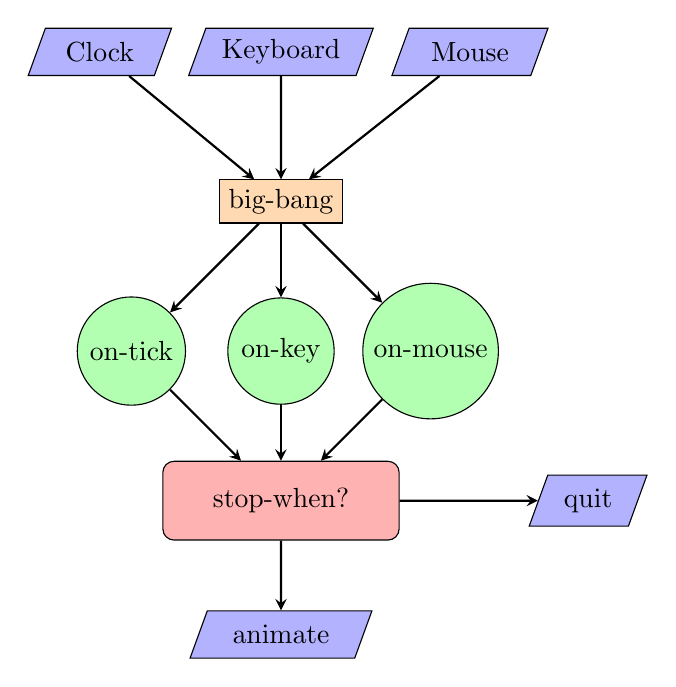
\begin{tikzpicture}[node distance=1.9cm]
      % \node (start) [startstop] {Start};
      \node (in1) [io] {Keyboard};
      \node (in2) [io, right of = in1, xshift=0.5cm] {Mouse};
      \node (in3) [io, left of = in1, xshift=-0.4cm] {Clock};

      \node (pro1) [process, below of=in1] {big-bang};
      % \node (pro2) [process, right of=pro1] {f2};

      \node (dec1) [decision, below of=pro1] {on-key};
      \node (dec2) [decision, right of = dec1] {on-mouse};
      \node (dec3) [decision, left of = dec1] {on-tick};

      \node (out1) [startstop, below of=dec1] {stop-when?};
      \node (out2) [io, below of=out1, yshift=0.2cm] {animate};
      \node (out3) [io, right of=out1, xshift=2cm] {quit};
      % \node (pro3) [process, right of=pro2] {...};
      % \node (out1) [io, right of=pro3] {Output};
      \draw [arrow] (in1) -- (pro1);
      \draw [arrow] (in2) -- (pro1);
      \draw [arrow] (in3) -- (pro1);

      \draw [arrow] (pro1) -- (dec1);
      \draw [arrow] (pro1) -- (dec2);
      \draw [arrow] (pro1) -- (dec3);
      
      \draw [arrow] (dec1) -- (out1);
      \draw [arrow] (dec2) -- (out1);
      \draw [arrow] (dec3) -- (out1);

      \draw [arrow] (out1) -- (out2);
      \draw [arrow] (out1) -- (out3);
    \end{tikzpicture}
  \end{center}
\end{frame}

\begin{frame}
  \frametitle{Our First Event Driven Program}
  With the big bang structure in mind, we can start writing our first big-bang
  program in Racket. It'll draw a square that starts by taking up the whole
  window and will shrink until it disappears.

  \begin{itemize}
  \item<2-> To start with this, we need a function
    that draws a square based on a numerical input.
  \item<3-> \mintinline{racket}{(define (number->square s) (square s "solid" "red")}
  \item<4-> In order to animate the square shrinking, we want to continually
    call \mintinline{racket}{number->square} with smaller values.
  \item<5-> \mintinline{racket}{(number->square 10)},  \mintinline{racket}{(number->square 5)}, \mintinline{racket}{(number->square 1)}
  \item<6-> Let's put it in Dr. Racket
  \end{itemize}
\end{frame}

\defverbatim[colored]\firstBigBang{
\begin{minted}{racket}
    (big-bang 100
        [to-draw number->square]
        [on-tick sub1]
        [stop-when zero?])
\end{minted}
}

\begin{frame}
  \frametitle{Using big-bang}
  Let's start with a very rough start to our program:
  \begin{itemize}
  \item<2-> \mintinline{racket}{(big-bang 100 [to-draw number->square])}
  \item<3-> When we close the program, Racket produces 100, the final state
    of our program
  \item<4-> Having a red square fill a frame until we close it isn't very interesting.
  \item<5-> In order to make a more interesting program, we need to write code
    that \emph{produces a new world state} based on clock ticks.
  \item<6-> There's a lot to unpack here:
    \firstBigBang
  \item<7-> First, note that the effectful code for checking system time, etc.
    is abstracted away by big-bang
  \end{itemize}
\end{frame}

\begin{frame}
  \frametitle{Unpacking This Program}
  Let's start from the top:
  \begin{itemize}
  \item<2-> \mintinline{racket}{(big-bang 100}
  \item<3-> \emph{And God said, ``Let there be \textcolor{red}{\underline{100}}``}
  \item<4-> \mintinline{racket}{[to-draw number->square]}
  \item<5-> The action taken by the universe is to draw a square, dependent upon
    the current state
  \item<6-> \mintinline{racket}{[on-tick sub1]}
  \item<7-> At each step of the universe's development, we subtract 1 from
    the current state of the universe. 100, 99, ..., 1, 0
  \item<8-> \mintinline{racket}{[stop-when zero?]}
  \item<9-> The actions taken by the universe end when the state of the universe
    is 0.
  \item<10-> And then Racket shuffles off this mortal coil.
  \end{itemize}
\end{frame}

\begin{frame}
  \frametitle{Action, Inaction, and Interaction}
  The last program was a simple start to event-driven program, but the only
  event it handled was the flow of time!
  \begin{itemize}
  \item<2-> So let's get a program with some (inter)action!
  \item<3-> We will want to reset the universe to 100, every time you (the god of this universe) presses a key. (action!)
  \item<4-> Otherwise, the universe decrements as usual. (inaction!)
  \item<5-> So, we will need to use the \mintinline{racket}{on-key} event handler.
  \item<6-> But how do we reset the state of the universe?
  \item<7-> Notice that our other handlers like in \mintinline{racket}{[on-tick sub1]} take a \emph{function} to create the new universe state.
  \item<8-> Help me write a reset function!
  \end{itemize}
\end{frame}

\begin{frame}
  \frametitle{Endgame}
  Ok, so (hopefully) the function we came up with looked something like this:
  \begin{itemize}
  \item<2-> \mintinline{racket}{(define (reset state key-event) 100)}
  \item<3-> Yay time travel!
  \item<4-> Our function doesn't actually care about the current state of the
    universe or the specific key that was pressed
  \item<5-> But obviously, we can think of situations where that would matter...
  \item<6-> Name some!
  \end{itemize}
\end{frame}

\begin{frame}
  \frametitle{Briefly Sidetracked}
  Alright, so now we realize we can write Doom as a big-bang program, right?
  \\\\
  %\begin{center}
  \includegraphics[width=\textwidth]{images/Carmack.png}
  %\end{center}
\end{frame}

\defverbatim[colored]\squareReset{
\begin{minted}{racket}
(big-bang 100
    [to-draw number->square]
    [on-tick sub1]
    [stop-when zero?]
    [on-key reset])
\end{minted}
}

\begin{frame}
  \frametitle{Back to the Future}
  With our reset function defined, we can finish our new big-bang
  program as:
  \pause
  \squareReset
  \begin{itemize}
  \item<3-> Basically, when the state of the universe is reset, the state
    passed to the to-draw event handler is 100, and so a large square is
    drawn again.
  \item<4-> From here, normal clock ticks make sure that the state of the universe
    is decremented.
  \item<5-> Any key press resets the state.
  \item<6-> Unless we the state of the universe reaches 0 and ends.
  \end{itemize}
\end{frame}

\defverbatim[colored]\generalForm{
\begin{minted}{racket}
(big-bang cw0
  [on-tick tock]
  [on-key ke-h]
  [on-mouse me-h]
  [to-draw render]
  [stop-when end?]
  ...)
\end{minted}
}

\begin{frame}
  \frametitle{Analyzing big-bang}
  In some sense, we can think of a big-bang program as a \emph{stream}
  of function calls that produce world states which are threaded into the next
  function call. Here's a general form of big-bang:
  \pause
  \generalForm
  \begin{itemize}
    \item<3-> This defines 3 event handlers:
      \begin{enumerate}
      \item<4-> Clock events for every tick are handled by: tock
      \item<5-> Key events are handled by: ke-h
      \item<6-> Mouse events are handled by: me-h
      \end{enumerate}
    \item<7-> The programs stops when end? returns true
  \end{itemize}
\end{frame}

\begin{frame}
  \frametitle{Analyzing big-bang (cont.)}
  Our render function draws something (or produces a gui)
  at the end of each tick as a result of the current state. tock
  produces the next world state.
  \begin{itemize}
  \item<2-> Our event handling functions tock, ke-h, and me-h will supercede tick events and produce the next world states.
  \item<3-> If two events happen in simultaneously, Racket will arbitrarily order them.
  \item<4-> Here's a visualization of the event pipeline:
  \item<5-> \includegraphics[width=0.7\textwidth]{images/event-pipeline.png}
  \end{itemize}
\end{frame}

\defverbatim[colored]\threading{
\begin{minted}{racket}
(define cw1 (ke-h cw0 "a"))
(define cw2 (tock cw1))
(define cw3 (me-h cw2 90 100 "button-down"))
\end{minted}
}

\begin{frame}
  \frametitle{Analyzing big-bang (cont.)}
  Let’s interpret this table with the specific sequence of events: the user presses the “a” key, then the clock ticks, and finally the user clicks the mouse to trigger a “button down” event at position (90,100).
  \begin{enumerate}
  \item<2-> cw1 is the result of (ke-h cw0 "a");
  \item<3-> cw2 is the result of (tock cw1); and
  \item<4-> cw3 is the result of (me-h cw2 90 100 "button-down").
  \end{enumerate}
  \pause
  And a sequence of clock ticks is simply:
  \mintinline{racket}{(tock (tock (tock cw0)))}
  \pause
  \\\\
  To inspect the state at a certain point, you can add a stop function that
  produces 0 and ends the program. You can then look at the last point animated:
  \mintinline{racket}{(define (stop state key) 0)}
\end{frame}

\begin{frame}
  \frametitle{Take a Breath}
  \huge We covered a lot. It'll take a while and some practice  for it all to sink in. Next we move on to laws governing program design. This will make it easier
  to think about writing the types of programs covered.
\end{frame}
\end{document}


%%% Local Variables:
%%% mode: latex
%%% TeX-master: t
%%% End:
